\documentclass[11pt,a4paper]{ctexart}
\usepackage{geometry}
\usepackage{graphicx}
\usepackage{subfigure}
\usepackage{amsmath}
\usepackage{multirow}
\usepackage{listings}
\usepackage[colorlinks, linkcolor=black, anchorcolor=black, citecolor=black]{hyperref}

\CTEXsetup[format={\Large\bfseries}]{section}
\geometry{left=1in, right=1in, top=1in, bottom=1in}
\begin{document}
\title{数值分析与算法 \hspace{0.1in} 大作业1}
\author{罗云鹏 \hspace{0.1in} 自 64 \hspace{0.1in}2016011470}
\maketitle
\tableofcontents
\newpage

\section{需求分析}
给定人脸图片,及其68个关键点坐标,设计程序,将一个图片中人脸变形,匹配到另一个人脸的关键点上。

\section{方案设计}
使用薄板样条模型,得到一个图像到另一个图像的变形函数。
对于一个空白图像的每一个点,使用变形函数,即可获得此点在原图中的对应坐标。
再使用最近临插值、双线性插值或者双三次插值,即可计算得到此点的值。

\section{方案基本原理}
为对人脸进行变形,首先应当得到从原始坐标到目标图像坐标的变形函数$$(x', y') = f(x, y)$$

由于人脸关键点较多,两图像关键点间一一对应,使得图形的变形过程较为复杂,难以用显式的数学公式表达。
使用薄板样条模型,寻找一个通过所有控制点的光滑曲面$f(x, y)$,使能量函数
$$I_f = \iint\limits_{R^2}\left(\left( \dfrac{\partial^2 f}{\partial x^2}\right)^2 + 2 \left( \dfrac{\partial^2 f}{\partial x \partial y}\right)^2 + \left( \dfrac{\partial^2 f}{\partial y^2}\right)^2 \right) dx dy$$
取得最小,此时$f(x, y)$可作为一个变形函数。
具体计算过程在PPT中已经给出,此处不再赘述。

可将图片看作一个关于坐标的二元函数$I(x, y)$。
若有人脸图像A与B以及其特征点坐标文件,欲对A图进行变形,使得特征点位置符合B图位置。
先建立一个空白图像C,并求得由B图到A图的变形函数。
对于空白图像C中每一个像素点,将其坐标$(x, y)$代入变形函数,求得其在A图中对应的坐标$(x', y')$。
应当注意的是,此处求得的$(x', y')$并不是整数值,故应当使用插值的方法,根据图A中$(x', y')$附近的像素点通过插值求得此点的值$I^*(x', y')$。
最后,将结果赋予图C中$(x, y)$位置的像素。

插值过程中,可采用最近邻、双线性、双三次的方法,不同方法带来的误差也会不同。

\section{误差分析}
\subsection{舍入误差}
计算过程中主要使用整型与浮点数(double)两种变量。
整型的舍入误差为$\Delta_i \le 0.5$,double类型浮点数的有效数字为10位,舍入误差相对小得多,可忽略。
对于三种插值方法的舍入误差具体分析见后。

\subsection{最近邻插值}
\subsubsection{舍入误差}
最近邻插值在计算时,直接取最近像素点的值,故舍入误差$\epsilon = \Delta_i \le 0.5$。

\subsubsection{方法误差}
令坐标$(x', y') = (i + u, j + v)$,其中$i, j$为整数,$u, v \in (-0.5, 0.5)$,则$I^*(i + u, j + v) = I(i, j)$。

由二元函数的中值定理,
\begin{align*}
\lvert e^*\rvert &= \lvert I^*(i + u, j + v) - I(i + u, j + v) \rvert\\
&= \lvert I(i, j) - I(i + u, j + v) \rvert \\
&= \lvert \dfrac{\partial I}{\partial x}(i + \theta u, j + \theta v) u + \dfrac{\partial I}{\partial y}(i + \theta u, j + \theta v) v \rvert
\end{align*}
其中$\theta \in [0, 1]$。不妨假设$\max \dfrac{\partial I}{\partial x}(i + \theta u, j + \theta v) = M_1$,$\max \dfrac{\partial I}{\partial y}(i + \theta u, j + \theta v) = M_2$,则有
$$\epsilon^* \le 0.5M_1 + 0.5M_2$$

\subsection{双线性插值}
\subsubsection{舍入误差}
双线性插值公式为
$$
I(i + u, j + v) = 
\begin{bmatrix}
    1-u & u
\end{bmatrix}
\begin{bmatrix}
    I(i, j) & I(i, j + 1) \\
    I(i + 1, j) & I(i + 1, j + 1)
\end{bmatrix}
\begin{bmatrix}
    1-v \\
    v
\end{bmatrix}
$$
其中$u, v \in [0, 1)$。

则有
\begin{align*}
&\epsilon =
\begin{bmatrix}
    1-u & u
\end{bmatrix}
\begin{bmatrix}
    \Delta_i & \Delta_i \\
    \Delta_i & \Delta_i
\end{bmatrix}
\begin{bmatrix}
    1-v \\
    v
\end{bmatrix} \\
&= \Delta_i [uv + (1-u)v + (1-v)u + (1-u)(1-v)] \\
&= \Delta_i \le 0.5
\end{align*}

\subsubsection{方法误差}
不妨设图像值函数二阶可导,且$M_x$为此区域图像在x轴方向上的二阶偏导最大绝对值,$M_y$为此区域图像在y轴方向上的二阶偏导最大绝对值。

双线性插值可认为是先在x轴方向上做线性插值,再在y轴方向上做线性插值,则有
$$I^*(i + u, j + 1) = uI(i + 1, j + 1) + (1 - u)I(i, j + 1)$$
$$I^*(i + u, j) = uI(i + 1, j) + (1 - u)I(i, j)$$
不妨设
$$I^*(i + u, j) = I(i + u, j) - R_{x1}$$
$$I^*(i + u, j + 1) = I(i + u, j + 1) - R_{x2}$$
两点处插值余项满足
$$R_x \le \lvert \dfrac{M_x}{2!} (x - i)(x - i - 1)\rvert \le \dfrac{M_x}{8}$$
则有
\begin{align*}
I^*(i + u, j + v) &= v I^*(i + u, j + 1) + (1 - v) I^*(i + u, j)\\
&= v\left[ I(i + u, j + 1) - R_{x2} \right] + (1 - v)\left[ I(i + u, j) - R_{x1} \right]\\
&= vI(i + u, j + 1) + (1 - v)I(i + u, j) - vR_{x2} - (1 - v)R_{x1}\\
&\le \lvert vI(i + u, j + 1) + (1 - v)I(i + u, j) \rvert + \lvert R_x \rvert\\
&\le \frac{1}{8}M_x + \frac{1}{8}M_y
\end{align*}

\subsection{双三次插值}
\subsubsection{舍入误差}
双三次插值的公式为
\begin{align*}
    &I^*(i + u, j + v) = ABC^T \\
    &A = 
    \begin{bmatrix}
        S(u + 1) & S(u) & S(u - 1) & S(u - 2)
    \end{bmatrix}\\
    &B = I(i-1:i+2, j-1:j+2)\\
    &C = 
    \begin{bmatrix}
        S(v + 1) & S(v) & S(v - 1) & S(v - 2)
    \end{bmatrix}
\end{align*}

其中
\begin{equation*}
S(x) = \left\{
\begin{aligned}
    &1 - 2\lvert x \rvert^2 + \lvert x \rvert^3 & \lvert x \rvert \le 1 \\
    &4 - 8\lvert x \rvert + 5 \lvert x \rvert^2 - \lvert x \rvert^3 & 1 < \lvert x \rvert < 2 \\
    &0 & otherwise
\end{aligned}
\right.
\end{equation*}

因为
$$S(u+1) + S(u) + S(u-1) + S(u-2) = 1$$

易得
$$\epsilon = \Delta_i \le 0.5$$

\subsubsection{方法误差}
不妨设图像值函数四阶可导,且$M_x$为此区域图像在x轴方向上的四阶偏导最大绝对值,$M_y$为此区域图像在y轴方向上的四阶偏导最大绝对值。
双三次插值过程可看作先在x轴方向上做三次样条插值,再利用计算出的结果在y轴方向上做三次样条插值。
由教材结论,有
$$R_x \le \dfrac{5}{384} M_x $$

则在x轴方向上做三次样条插值后,有结果
$$I^*(i + u, y) = I(i + u, y) + R_x$$

因此,与双线性插值的误差分析类似,在$(i + u, j + v)$处插值余项满足
\begin{align*}
R(i + u, j + v) &\le \lvert I^*(i + u, j - 2) S(v + 1) + I^*(i + u, j - 1) S(v) \\
&+ I^*(i + u, j) S(v - 1) + I^*(i + u, j + 1) S(v - 2) \rvert \\
&= \lvert I(i + u, j - 2) S(v + 1) + I(i + u, j - 1) S(v) \\
&+ I(i + u, j) S(v - 1) + I(i + u, j + 1) S(v - 2) \\
&+ \left[ S(v + 1) + S(v) + S(v - 1) + S(v - 2) \right] M_x \rvert \\
&\le \dfrac{5}{384} (M_y + M_x)
\end{align*}

\section{程序使用及结果}
程序使用说明见 ./picture/README.md

效果如下,在输出图片中标出了特征点位置(使用给出的特征点数据,以及使用特征点识别算法)

\clearpage
\begin{lstlisting}[frame=single]
./FaceMatch.exe -s 8.jpg -t 6.jpg -1 8.txt -2 6.txt -ap
\end{lstlisting}

\begin{figure}[!htp]
    \begin{center}
        \subfigure[最近邻插值]{ 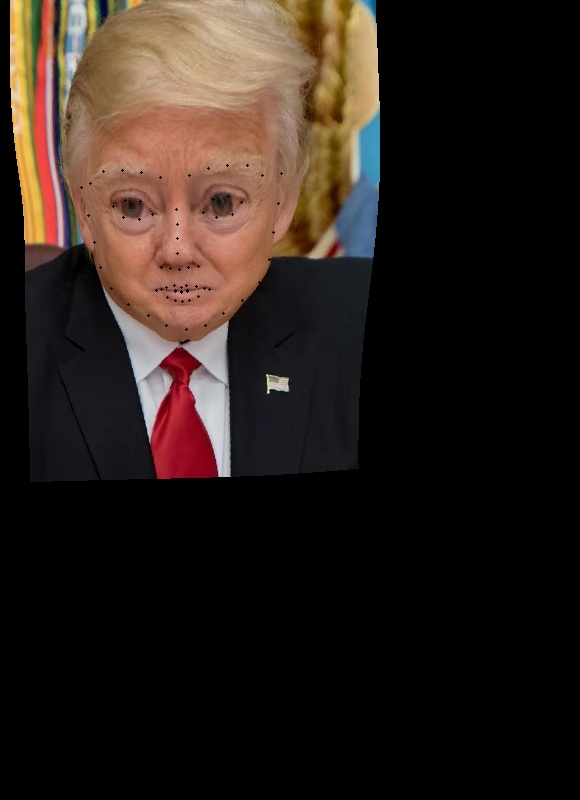
\includegraphics[width=0.3\textwidth]{./pic/8_6_neighbour.jpg}}
        \subfigure[双线性插值]{ 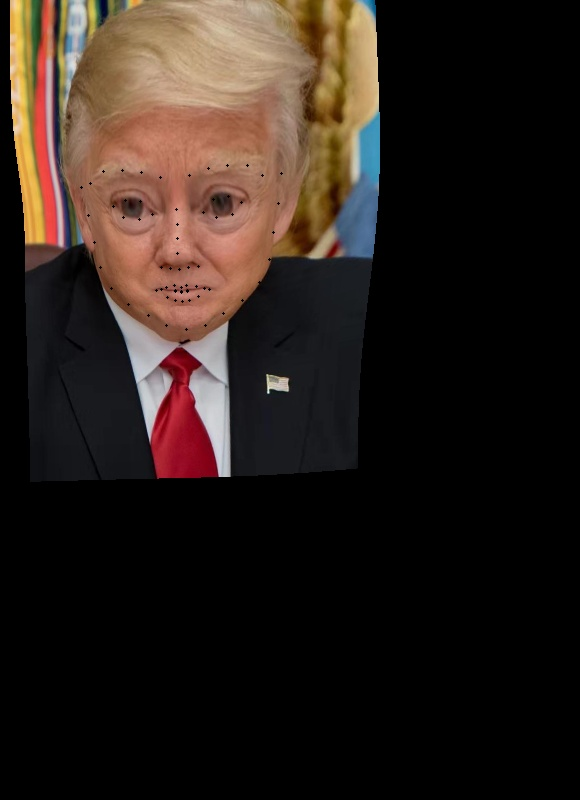
\includegraphics[width=0.3\textwidth]{./pic/8_6_bilinear.jpg} }
        \subfigure[双三次插值]{ 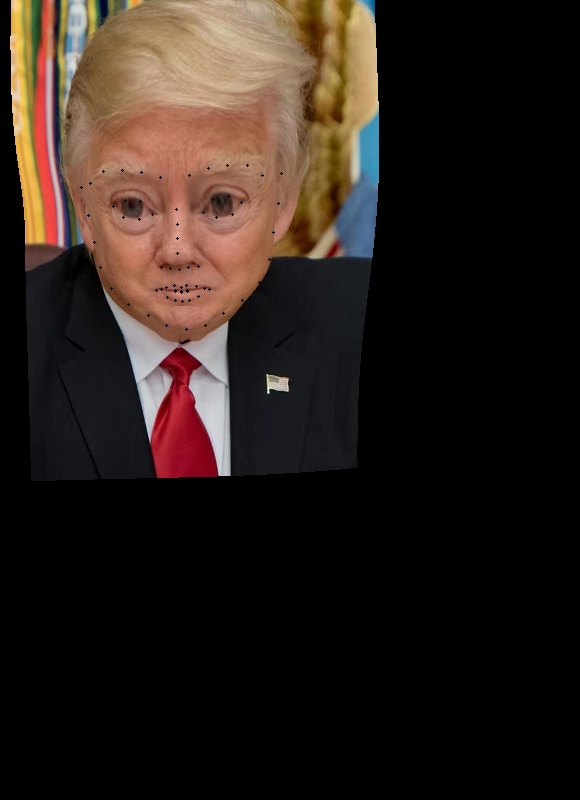
\includegraphics[width=0.3\textwidth]{./pic/8_6_bicubic.jpg} }
        \subfigure[原图]{ 
\includegraphics[width=0.3\textwidth]{./pic/8.jpg} }
        \subfigure[目标图像]{ 
\includegraphics[width=0.3\textwidth]{./pic/6.jpg} }
    \end{center}
    \caption{8.jpg 到 6.jpg,使用给出的坐标点}
    \label{fig:p1}
\end{figure}

\clearpage

\begin{lstlisting}[frame=single]
./FaceMatch.exe -s test.jpg -t 8.jpg -1 anything -2 anything -apd
\end{lstlisting}

\begin{figure}[!htp]
    \begin{center}
        \subfigure[最近邻插值]{ 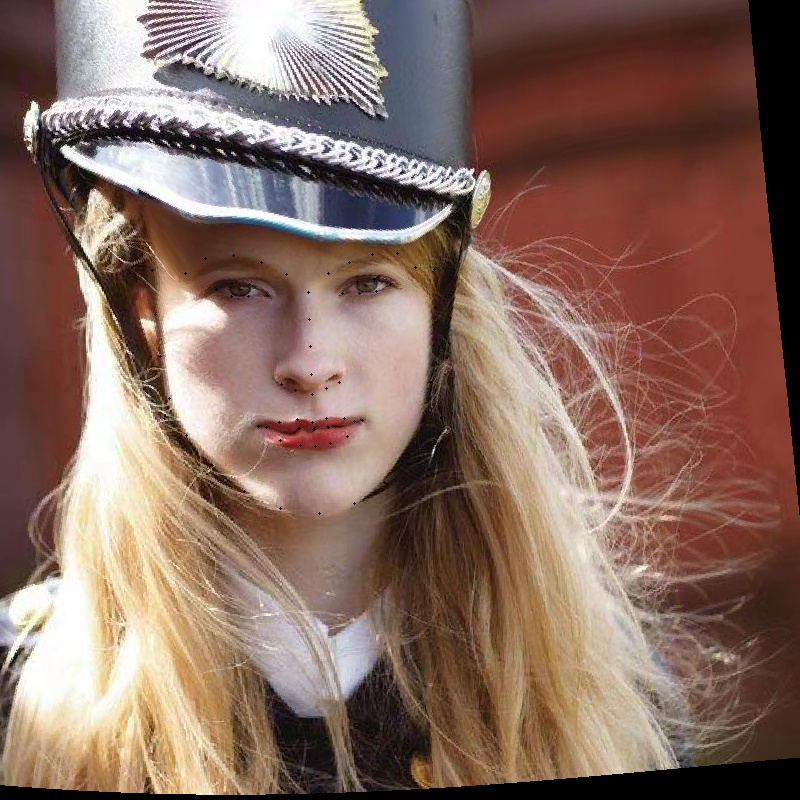
\includegraphics[width=0.3\textwidth]{./pic/test_8_neighbour.jpg}}
        \subfigure[双线性插值]{ 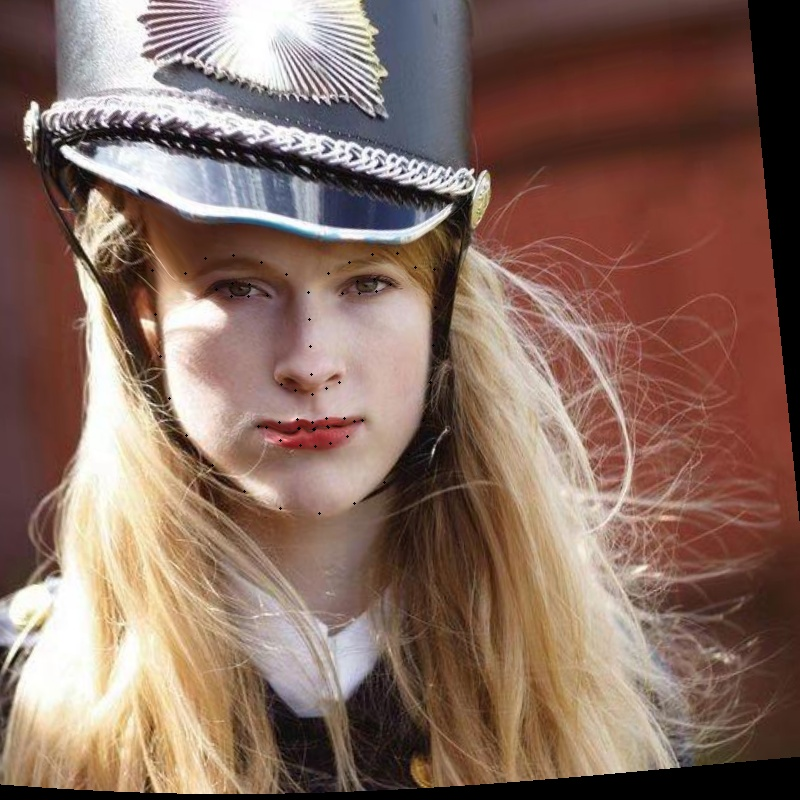
\includegraphics[width=0.3\textwidth]{./pic/test_8_bilinear.jpg} }
        \subfigure[双三次插值]{ 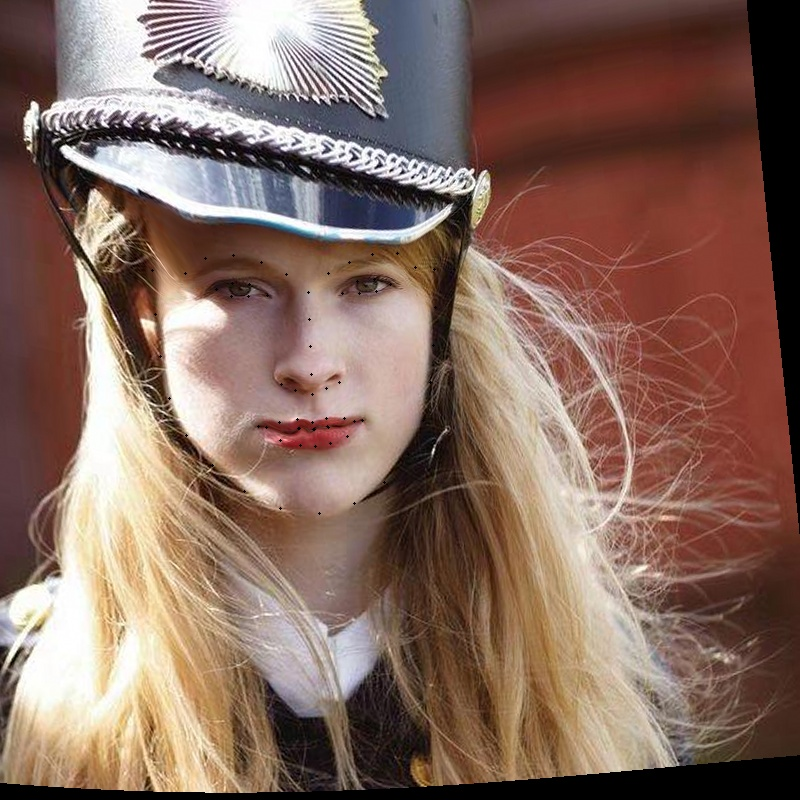
\includegraphics[width=0.3\textwidth]{./pic/test_8_bicubic.jpg} }
        \subfigure[原图]{ 
\includegraphics[width=0.3\textwidth]{./pic/test.jpg} }
        \subfigure[目标图像]{ 
\includegraphics[width=0.3\textwidth]{./pic/8.jpg} }
    \end{center}
    \caption{test.jpg 到 8.jpg, 使用特征点检测算法}
    \label{fig:p2}
\end{figure}

\end{document}
